\documentclass{article}
\usepackage[utf8x]{inputenc}
\usepackage{graphicx}
\usepackage{tikz, amsmath, amssymb, bm, color}
\usepackage{geometry}
\usetikzlibrary{calc}
\usetikzlibrary{shapes,arrows}
\usepackage{todonotes}
\usepackage[american]{circuitikz}
\usepackage{pgfplots}
\usepackage{epstopdf}
\usepackage{listings}
\usepackage{subcaption}
\usepackage{mwe}
\usepackage{float}
\usepackage{cleveref}
\usepackage{ragged2e} % For text alignment


\newenvironment{custom_itemize}{
\begin{itemize}
  \setlength{\itemsep}{0pt}
  \setlength{\parskip}{0pt}
  \setlength{\parsep}{0pt}
}{\end{itemize}}


%\usepackage{multicol} % Used for the two-column layout of the document


%\usepackage{bm}


\title{Preethi's ROIC analysis}
\author{Kees Kroep 4246373}


\begin{document}
%  \twocolumn[{%
% \begin{@twocolumnfalse}
  \maketitle
%   \end{@twocolumnfalse}
% }]

\section{setup}\label{sec:setup}
\begin{figure}[H]
\centering
\usetikzlibrary{shapes,snakes}
\tikzstyle{dot} = [draw,shape=circle,fill=black, scale =.2]
\tikzstyle{l_arrow} = [draw,fill = black, regular polygon,regular polygon sides=3, rotate=-90, anchor=south, scale=.5] 
\tikzstyle{l_text} = [anchor=south west]
\tikzstyle{r_arrow} = [draw,fill = black, regular polygon,regular polygon sides=3, rotate=90, anchor=south, scale=.5] 
\tikzstyle{r_text} = [anchor=south east]
\begin{tikzpicture}[scale=1.5, every node/.style={scale=1}]


\node[l_text] at (-3,1) {VDD 3.3 (1)};
\node[l_text] at (-3,0) {IN[8] (15)};
\node[l_text] at (-3,-1) {VSUB (16)};
\node[l_text] at (-3,-2) {VDD\_HV (17)};
\node[l_text] at (-3,-3) {GND\_HV (18)};

\node[l_arrow] at (-3,1) {};
\node[l_arrow] at (-3,0) {};
\node[l_arrow] at (-3,-1) {};
\node[l_arrow] at (-3,-2) {};
\node[l_arrow] at (-3,-3) {};

\node[r_text] at (0,1) {(25) gnd};
\node[r_text] at (0,0) {(26) VDD5};
\node[r_text] at (0,-1) {(27) Vg};
\node[r_text] at (0,-2) {(28) Rst[3]};
\node[r_text] at (0,-3) {(29) Rst[1]};
\node[r_text] at (0,-4) {(30) Rst[2]};
\node[r_text] at (0,-5) {(31) Res};
\node[r_text] at (0,-6) {(32) VB0[8]};
\node[r_text] at (0,-7) {(33) out[8]};
\node[r_text] at (0,-8) {(48) gnd};


\node[r_arrow] at (0,1) {};
\node[r_arrow] at (0,0) {};
\node[r_arrow] at (0,-1) {};
\node[r_arrow] at (0,-2) {};
\node[r_arrow] at (0,-3) {};
\node[r_arrow] at (0,-4) {};
\node[r_arrow] at (0,-5) {};
\node[r_arrow] at (0,-6) {};
\node[r_arrow] at (0,-7) {};
\node[r_arrow] at (0,-8) {};
\draw  (-3,2) rectangle (0,-8);




\draw (-3.5,-1) node[ground]{} to (-3,-1);
\draw (-3.5,-3) node[ground]{} to (-3,-3);
\draw (0.5,1) node[ground]{} to (0,1);
\draw (0.5,-8) node[ground]{} to (0,-8);
\draw (0.5,-3) node[ground]{} to (0,-3);
\draw (0.5,-4) node[ground]{} to (0,-4);

\draw (0.5,0.25) node[anchor=south]{$5\,V$} (0.5,0.25) node[tground]{} to (0.5,0)to (0,0); % VDD5
\draw (0.5,-0.75) node[anchor=south]{$4.5\,V$} (0.5,-0.75) node[tground]{} to (0.5,-1)to (0,-1); % Vg
\draw (-3.5,1.25) node[anchor=south]{$3.3\,V$} (-3.5,1.25) node[tground]{} to (-3.5,1)to (-3,1); % VDD3.3
\draw (-3.5,-1.75) node[anchor=south]{$5\,V$} (-3.5,-1.75) node[tground]{} to (-3.5,-2)to (-3,-2); %VDD_HV
\draw (-4.5,0.25) node[anchor=south]{$set$} (-4.5,0.25) node[tground]{} to (-4.5,0)to (-4.5,0); % IN[8]
\draw (0.5,-1.75) node[anchor=south]{$reset$} (0.5,-1.75) node[tground]{} to (0.5,-2)to (0,-2); % Rst[3]
\draw  (0,-5) to[R=$50\,k\Omega$](1.5,-5) to (1.5,-4.75) node[tground]{} (1.5,-4.75) node[anchor=south]{$5\,V$}; %res


\draw (-4.5,0) to [R=$20\,M\Omega$](-3,0);

\end{tikzpicture}
\caption{Schematic of breadbord}
\label{tkz:breadbord}
\end{figure}
\begin{figure}[H]
\centering
\tikzstyle{dot} = [draw,shape=circle,fill=black, scale =.3]
\tikzstyle{l_arrow} = [draw,fill = black, regular polygon,regular polygon sides=3, rotate=-90, anchor=south, scale=.5] 
\tikzstyle{l_text} = [anchor=south west]
\tikzstyle{r_arrow} = [draw,fill = black, regular polygon,regular polygon sides=3, rotate=90, anchor=south, scale=.5] 
\tikzstyle{r_text} = [anchor=south east]
\begin{tikzpicture}[scale=1, every node/.style={scale=1}]

\draw[dashed, color=gray]  (-0.5,5.5) rectangle (0.5,-2);
\fill[color=gray, opacity=.1]  (-0.5,5.5) rectangle (0.5,-2);
\node[align=center, anchor=south] at (0,5.5) {voltage\\limiter};

\draw[dashed, color=gray]  (1.25,5.5) rectangle (5.25,-2);
\fill[opacity=.1, color=gray]  (1.25,5.5) rectangle (5.25,-2);
\node[align=center, anchor=south] at (3.25,5.5) {integrator};



\draw[dashed, color=gray]  (5.75,5.5) rectangle (9.25,-2);
\fill[opacity=.1, color=gray] (5.75,5.5) rectangle (9.25,-2);
\node[align=center, anchor=south] at (7.5,5.5) {current mirrors};

%\draw (0,0) to node[nfet]{};

%\draw (0,0) to (mos1.s);
\node(Vg)[nfet, rotate=-90] at (0,2.5) {};
\node[pfet, rotate=-90] (Reset) at (2.5,2) {};
\node[pfet] (CM_H1) at (5,3) {};
\node[nfet] (CM_L1) at (5,-1) {};
\node[nfet] (CM_H2) at (7,3) {};
\node[nfet] (CM_L2) at (7,-1) {};
\node[nfet] (CM_H3) at (9,3) {};
\node[nfet] (CM_L3) at (9,-1) {};



\draw (-1,2.5) node[anchor=east]{IN[i]} to (Vg.S);
\draw (Vg.G) |- (0,4.5) node[anchor=south]{Vg};
\draw (Vg.B) |- (1,2.5) node[dot]{} |- (CM_H1.G); %top
\draw (1,2.5) |- (1,0.5)  to [C=$C_{fb}$](4,0.5) -| (CM_H1.D);
\draw (1.5,0.5) node[dot]{} -| (1.5,2) |- (Reset.B);
\draw (Reset.G) to (2.5,4.5) node[anchor=south]{Rst[3]};
\draw (Reset.D) -| (3.5,0.5) node[dot]{};
\draw (5,0.5) node[dot]{} to (CM_L1.D);
\draw (CM_L1.G) to (4,4.5) node[anchor=south]{Res}; 
\draw (CM_L1.S) to (CM_L2.S) to (7,-2.5) node[anchor=north]{gnd};
\draw (CM_H1.B) |- (CM_H2.D) to (7,4.5) node[anchor=south]{VDD3.3};
\draw (CM_L2.G) |- (4,0) node[dot]{};
\draw (5,0.5) -| (CM_H2.G);
\draw (CM_L1.B) to (CM_L1.S);
\draw (CM_L2.B) to (CM_L2.S);
\draw (CM_H2.B) to (CM_L2.D);
\draw (CM_H3.B) to (CM_L3.D);
\draw (1,3)node[dot]{} |- (8,4) |- (CM_H3.G);
\draw (CM_H3.D) |- (CM_H2.D) node[dot]{};
\draw (CM_L3.S) |- (CM_L2.S) node[dot]{};
\draw (CM_L3.G) |- (6,0) node[dot]{};
\draw (7,1.5)node[dot]{} to (10,1.5) node[anchor=west]{OUT[i]};
\draw (9,1)node[dot]{} to (10,1) node[anchor=west]{VBO[i]};



\end{tikzpicture}\caption{Schematic of ROIC channel}
\label{tkz:schematic_ROIC}
\end{figure}


\begin{figure}[h]
	\centering
	\includegraphics[width=0.6\linewidth]{fig/P1010158.JPG}
	\caption{setup overview}
	\label{fig:setup_overview}
\end{figure}

\begin{figure}[h]
	\centering
	\includegraphics[width=0.6\linewidth]{fig/P1010159.JPG}
	\caption{close-up}
	\label{fig:close-up}
\end{figure}

\clearpage

\section{Reset mode}
This test addresses the behavior of the circuit in reset mode. \Cref{tkz:schematic_ROIC_reset} shows the measured values during reset mode. Note that the input voltage is $2.4\,V$, which is important when calculating the input current. 

\input{tkz/ROIC_reset-on_tkz}


\section{Integrator}
This section aims to address the performance of the integrator. \Cref{tkz:integrator_test} shows the setup used for this test. Channel 8 was used, so the end of the $20\,M\Omega$ resistor is connected to IN[8], and the probe is connected to OUT[8]. 

\begin{figure}[H]
\centering

\usetikzlibrary{shapes,snakes}

\newcommand*{\Vg}{Vg\\ $\color{red}4.5\,V$}
\newcommand*{\Rst}{\textbf{Rst[3]}\\ $\color{blue}reset$} 
\newcommand*{\Res}{Res\\ $\color{red}0.86\,V$}
\newcommand*{\VDD}{VDD3.3\\ $\color{red}3.3\,V$}
\newcommand*{\IN}{$\color{blue}V_{in}$}
\newcommand*{\OUT}{$\color{blue}V_{out}$}
\newcommand*{\VBO}{\color{blue}\textbf{VBO[8]} $\color{red}1.4\,V$}
\newcommand*{\gnd}{gnd\\ $\color{red}0\,V$}
\newcommand*{\C}{$\color{blue}C$}




\tikzstyle{dot} = [draw,shape=circle,fill=black, scale =.3]
\tikzstyle{l_arrow} = [draw,fill = black, regular polygon,regular polygon sides=3, rotate=-90, anchor=south, scale=.5] 
\tikzstyle{l_text} = [anchor=south west]
\tikzstyle{r_arrow} = [draw,fill = black, regular polygon,regular polygon sides=3, rotate=90, anchor=south, scale=.5] 
\tikzstyle{r_text} = [anchor=south east]
\begin{tikzpicture}[scale=1, every node/.style={scale=1}]




\draw[dashed]  (-0.5,5.5) rectangle (0.5,-2);
\node[align=center, anchor=south] at (0,5.5) {voltage\\limiter};

\draw[dashed]  (1.25,5.5) rectangle (5.25,-2);
\node[align=center, anchor=south] at (3.25,5.5) {integrator};

\draw[dashed]  (5.75,5.5) rectangle (9.25,-2);
\node[align=center, anchor=south] at (7.5,5.5) {current mirrors};

%\draw (0,0) to node[nfet]{};

%\draw (0,0) to (mos1.s);
\node(Vg)[nfet, rotate=-90] at (0,2.5) {};
\node[nfet, rotate=-90] (Reset) at (2.5,2) {};
\node[pfet] (CM_H1) at (5,3) {};
\node[nfet] (CM_L1) at (5,-1) {};
\node[nfet] (CM_H2) at (7,3) {};
\node[nfet] (CM_L2) at (7,-1) {};
\node[nfet] (CM_H3) at (9,3) {};
\node[nfet] (CM_L3) at (9,-1) {};



\draw (-1,2.5) node[anchor=east, align=center]{} to (Vg.S);
\draw (Vg.G) |- (0,4.5) node[anchor=south, align=center]{\Vg};
\draw (Vg.B) |- (1,2.5) node[dot]{} |- (CM_H1.G); %top
\draw (1,2.5) |- (1,0.5)  to [C=\C](4,0.5) -| (CM_H1.D);
\draw (1.5,0.5) node[dot]{} -| (1.5,2) |- (Reset.B);
\draw (Reset.G) to (2.5,4.5) node[anchor=south, align=center]{\Rst};
\draw (Reset.D) -| (3.5,0.5) node[dot]{};
\draw (5,0.5) node[dot]{} to (CM_L1.D);
\draw (CM_L1.G) to (4,4.5) node[anchor=south, align=center]{\Res}; 
\draw (CM_L1.S) to (CM_L2.S) to (7,-2.5) node[anchor=north, align=center]{\gnd};
\draw (CM_H1.B) |- (CM_H2.D) to (7,4.5) node[anchor=south, align=center]{\VDD};
\draw (CM_L2.G) |- (4,0) node[dot]{};
\draw (5,0.5) -| (CM_H2.G);
\draw (CM_L1.B) to (CM_L1.S);
\draw (CM_L2.B) to (CM_L2.S);
\draw (CM_H2.B) to (CM_L2.D);
\draw (CM_H3.B) to (CM_L3.D);
\draw (1,3)node[dot]{} |- (8,4) |- (CM_H3.G);
\draw (CM_H3.D) |- (CM_H2.D) node[dot]{};
\draw (CM_L3.S) |- (CM_L2.S) node[dot]{};
\draw (CM_L3.G) |- (6,0) node[dot]{};
\draw (7,1.5)node[dot]{} to (10,1.5) node[anchor=west, align=center]{\OUT};
%\draw (9,1)node[dot]{} to (10,1) node[anchor=west, align=center]{\VBO};

\draw (-2.5,2.5)node[anchor=east, align=center]{\IN} to [R=$20\,M\Omega$](-1,2.5);


\end{tikzpicture}

\caption{Schematic of ROIC channel template}
\label{tkz:integrator_test}
\end{figure}


One can calculate the expected performance of the integrator using \cref{eq:t_vs_I}. The expected time to discharge the capacitance versus the measured time is plotted in \cref{fig:e_vs_m}. The slope of the $450\,fF$ and $350\,fF$ appear to be reasonably similar to the expected slope, but the $150\,fF$ and especially $50\,fF$ ones are way off. During some testing I found that adding approximately $90\,fF$ to both of those would make the measured and expected values match. It is also interesting to see the current limiting properties of the device in action. All four configurations limit at a $\delta V/\delta t=1.2\cdot10^6$, and with a resistanceof $20\,M\Omega$, this gives a current limitation of $50\,mA$.

\begin{align}
	\delta q&=C\cdot \delta V\\
	I&=\frac{V_{in}-V_0}{R}\\
	\delta t&=\frac{\delta q}{I}\\
	\frac{\delta V}{\delta t}&=\frac{I}{C}=\frac{V_{in}-V_0}{RC}\label{eq:t_vs_I}
\end{align}


\begin{figure}
	\centering
	\begin{subfigure}[b]{0.475\textwidth}
	    \centering
	    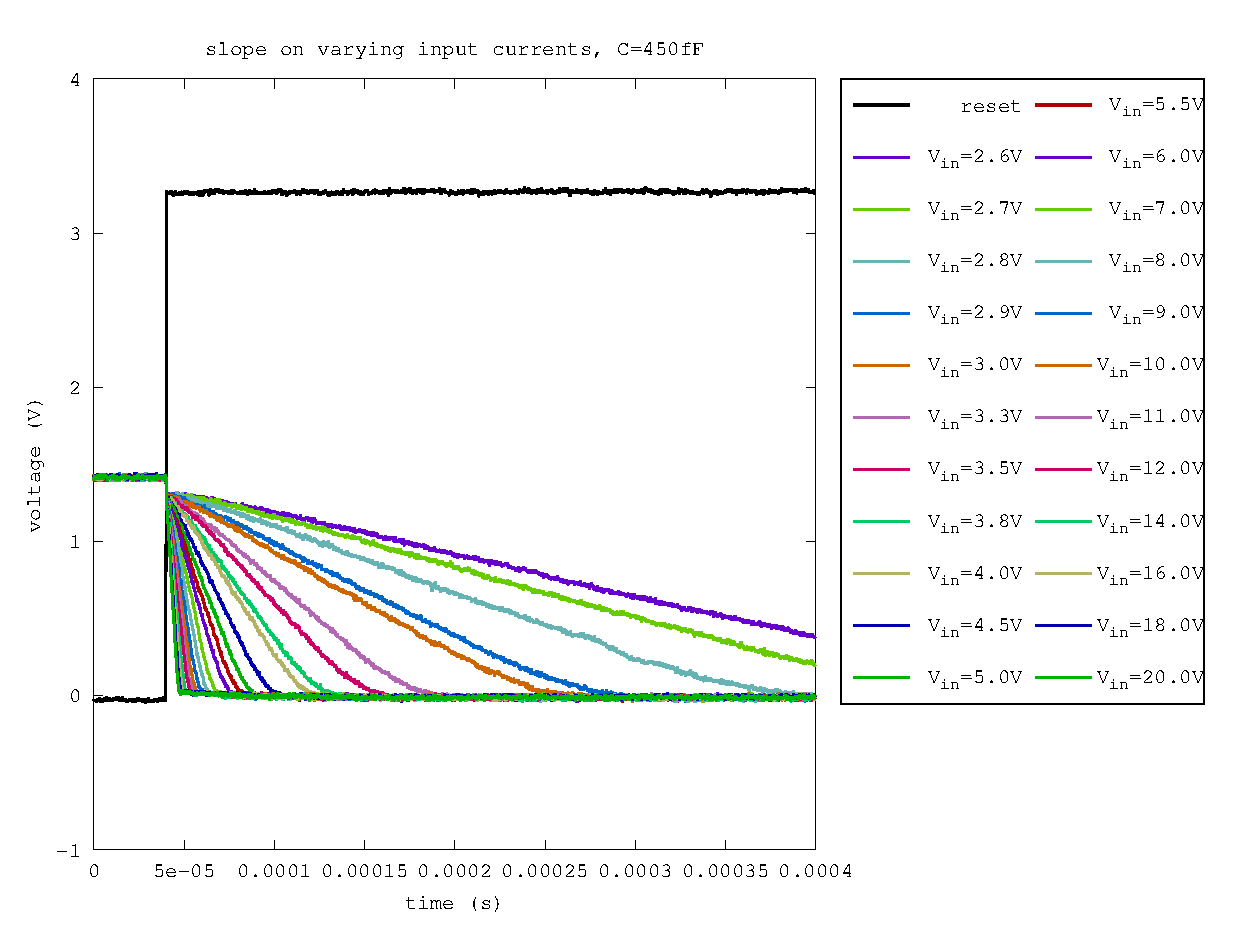
\includegraphics[width=\textwidth]{fig/slope_450fF.eps}
	    \caption[Network2]%
	    {$C=450\,fF$}    
	    \label{fig:slopes_450fF}
	\end{subfigure}
	\hfill
	\begin{subfigure}[b]{0.475\textwidth}  
	    \centering 
	    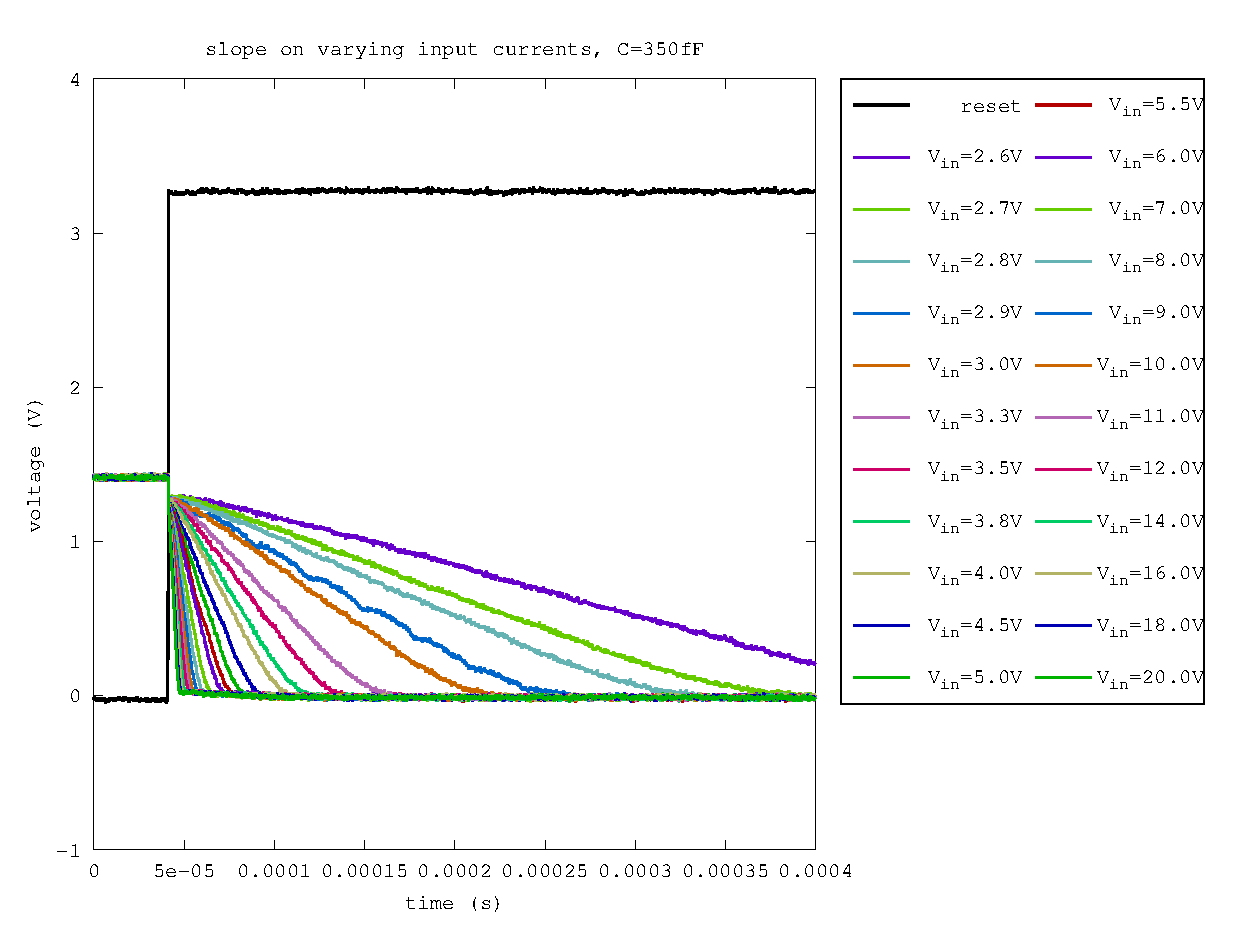
\includegraphics[width=\textwidth]{fig/slope_350fF.eps}
	    \caption[]%
	    {$C=350\,fF$}    
	    \label{fig:slopes_350fF}
	\end{subfigure}
	\vskip\baselineskip
	\begin{subfigure}[b]{0.475\textwidth}   
	    \centering 
	    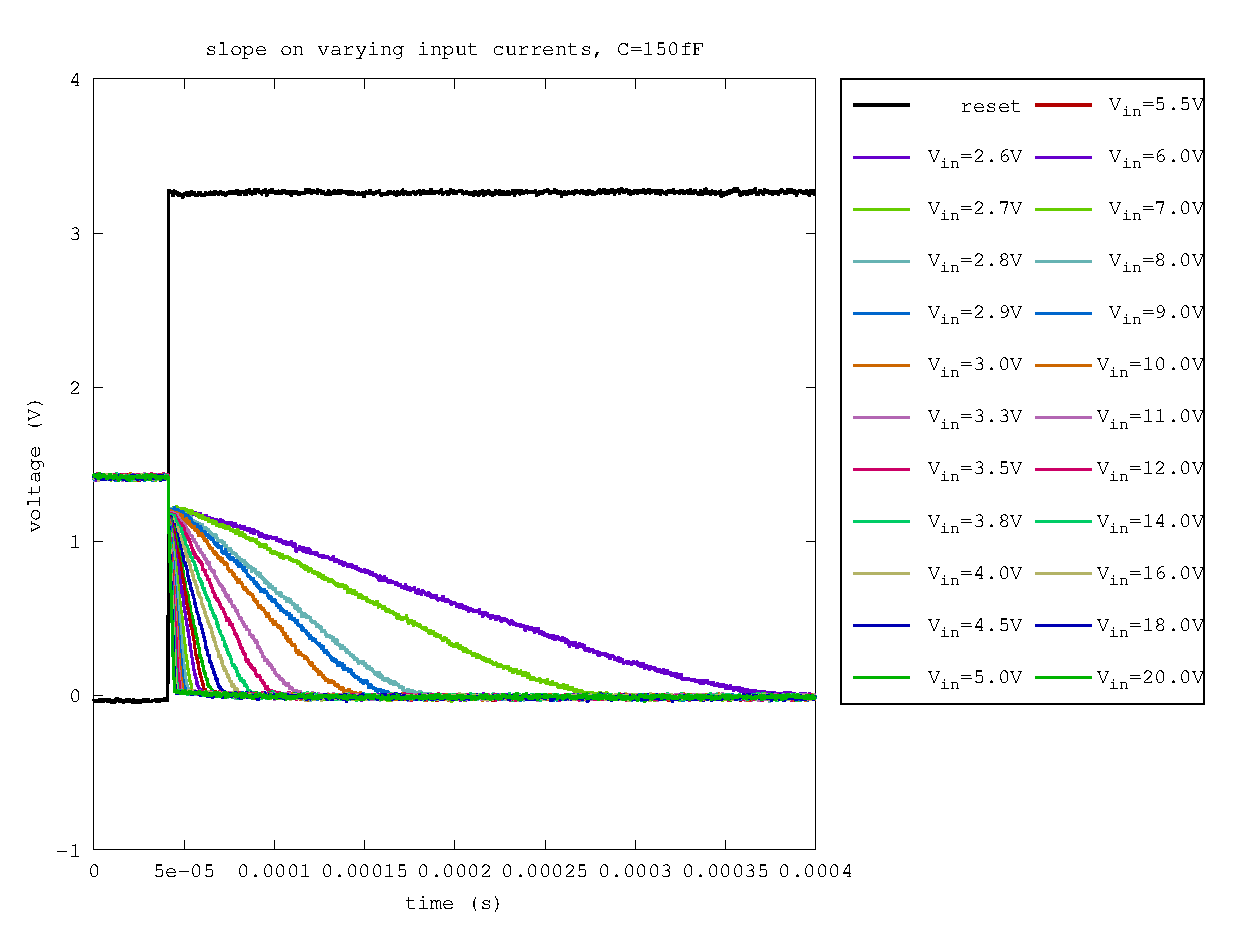
\includegraphics[width=\textwidth]{fig/slope_150fF.eps}
	    \caption[]%
	    {$C=150\,fF$}    
	    \label{fig:slopes_150fF}
	\end{subfigure}
	\quad
	\begin{subfigure}[b]{0.475\textwidth}   
	    \centering 
	    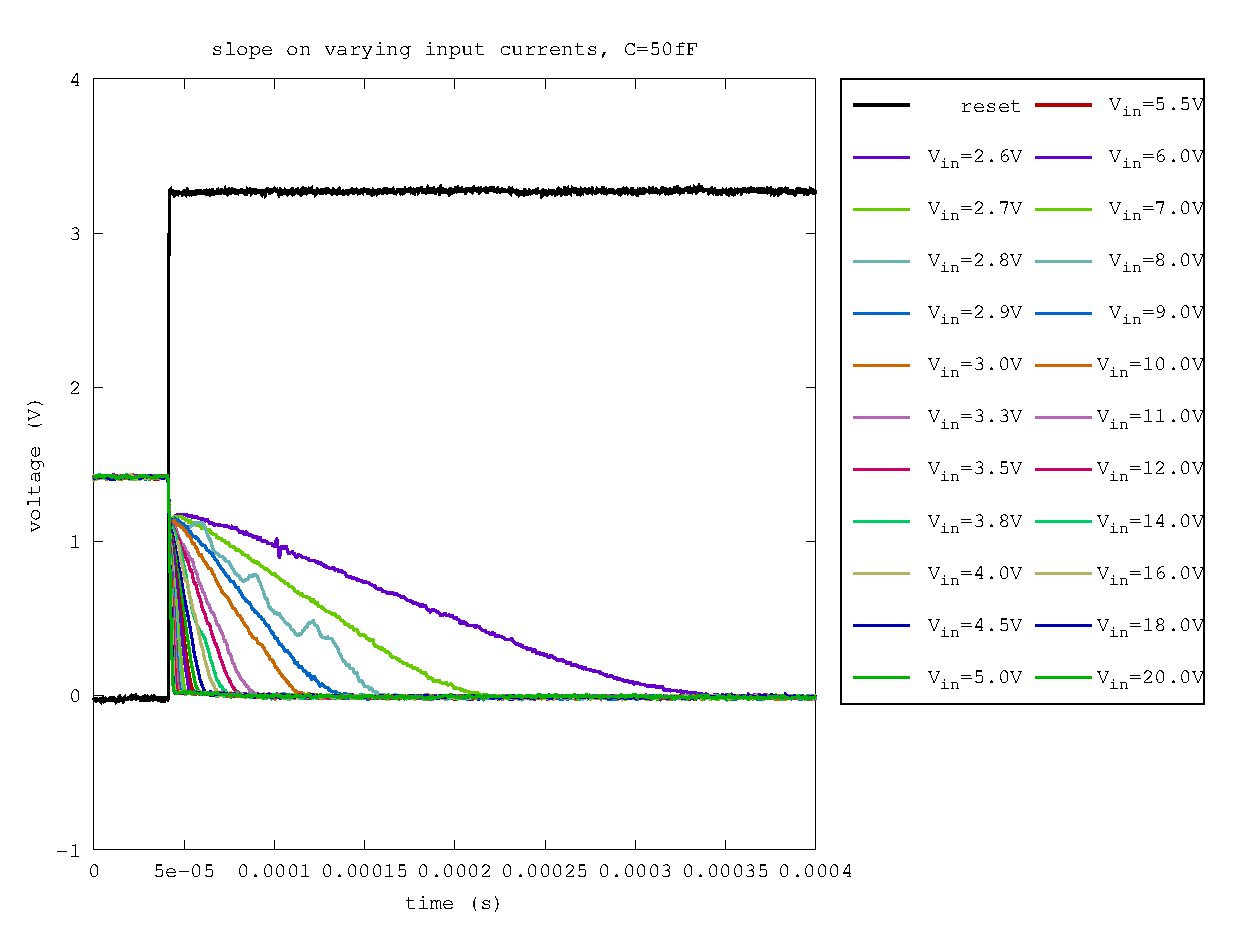
\includegraphics[width=\textwidth]{fig/slope_50fF.eps}
	    \caption[]%
	    {$C=50\,fF$}    
	    \label{fig:slopes_50fF}
	\end{subfigure}
	\caption{Expected versus measured charge up times for different input voltages. The input voltage is connected to the input through a resistor of $20\,M\Omega$}
	\label{fig:slopes}
\end{figure}

\begin{figure}
	\centering
	\begin{subfigure}[b]{0.475\textwidth}
	    \centering
	    \includegraphics[width=\textwidth]{fig/vin_vs_time_sat_450fF.eps}
	    \caption[Network2]%
	    {$C=450\,fF$}    
	    \label{fig:e_vs_m_450fF}
	\end{subfigure}
	\hfill
	\begin{subfigure}[b]{0.475\textwidth}  
	    \centering 
	    \includegraphics[width=\textwidth]{fig/vin_vs_time_sat_350fF.eps}
	    \caption[]%
	    {$C=350\,fF$}    
	    \label{fig:e_vs_m_350fF}
	\end{subfigure}
	\vskip\baselineskip
	\begin{subfigure}[b]{0.475\textwidth}   
	    \centering 
	    \includegraphics[width=\textwidth]{fig/vin_vs_time_sat_150fF.eps}
	    \caption[]%
	    {$C=150\,fF$}    
	    \label{fig:e_vs_m_150fF}
	\end{subfigure}
	\quad
	\begin{subfigure}[b]{0.475\textwidth}   
	    \centering 
	    \includegraphics[width=\textwidth]{fig/vin_vs_time_sat_50fF.eps}
	    \caption[]%
	    {$C=50\,fF$}    
	    \label{fig:e_vs_m_50fF}
	\end{subfigure}
	\caption{Expected versus measured charge up times for different input voltages. The input voltage is connected to the input through a resistor of $20\,M\Omega$.}
	\label{fig:e_vs_m}
\end{figure}

\end{document}












